\chapter{ម៉ាសុីន}
    \section{លំនាំអាដ្យាបាទិច}
    \begin{definition}
    	លំនាំអាដ្យាបាទិច ជាលំនាំដែលថាមពលកម្តៅមិនប្តូរជាមួយមជ្ឈដ្ឋានក្រៅ(មិនស្រូប និងមិនបញ្ចេញកម្តៅ) ឬមានតម្លៃថេរជានិច្ច $\left(\Delta Q=0\right)$។ តាមច្បាប់ទីមួយទែម៉ូឌីណាមិចយើងបានៈ $W=-\Delta U$។
    \end{definition}
    \begin{example}
    	\begin{enumerate}[m]
    		\item កាលណាឧស្ម័នត្រូវបានបណ្ណែនតាមបែបអាដ្យាបាទិច កម្មន្តបានធ្វើទៅលើឧស្ម័ននោះគឺ $640J$។\\ គណនាបម្រែបម្រួលថាមពលក្នុងរបស់ឧស្ម័ន។
    		\item ក្នុងប្រព័ន្ធត្រមោចមួយ បើថាមពលក្នុងថយចុះ $500J$ តើកម្មន្តដែលបំពេញដោយប្រព័ន្ធនោះស្មើនឹងប៉ុន្មាន?
    	\end{enumerate}
    \end{example}
    \section{ម៉ាសុីនទ្រឹស្តី(ម៉ាសុីនកាណូ, ម៉ាសុីនអុីដេអាល់)}
    \subsection{ម៉ាសុីនកម្តៅ}
    \begin{definition}
    	\emph{\kml ម៉ាសុីនកម្តៅ{\en(Heat Engine)}} ជាឧបករណ៍ ឬម៉ូទ័រទាំងឡាយណាដែលបម្លែងថាមពលកម្តៅទៅជាកម្មន្ត។\\ ដែលគេអាចហៅយ៉ាងខ្លីថា "ម៉ាសុីន" មានម៉ាសុីនម៉ូតូ ម៉ាសុីនឡាន ម៉ាសុីនភ្លើង។ល។
    \end{definition}
    \begin{minipage}[l]{.5\textwidth}
    	ឧទាហរណ៍គំរូនៃប្រភេទឧបករណ៍នេះ គឺម៉ាសុីនចំហាយទឹកដែលអាចសង្ខេបយ៉ាងងាយបានដូចរូបខាងក្រោម។
    	ដំណើរការរបស់វាគឺដំបូងគេប្រើប្រាស់ឥតន្ធនៈដើម្បីបង្ហូរទឹកក្នុងឆ្នាំងដាំទឹក(ប្រភពធុងក្តៅ) ដែលបង្កើតឲ្យមានចំហាយ រួចហើយឲ្យចំហាយនោះចូលក្នុងម៉ាសុីនឡើងវិញដែលនៅពេលនោះវារីកមឌដោយអាចធាក់ពីស្តុងដើម្បីធ្វើកម្មន្ត(មើលរូប)។
    \end{minipage}
    \begin{minipage}[r]{.6\textwidth}
    	\begin{figure}[H]
    		\centering
    		\begin{tikzpicture}
    		\node at (0,0) {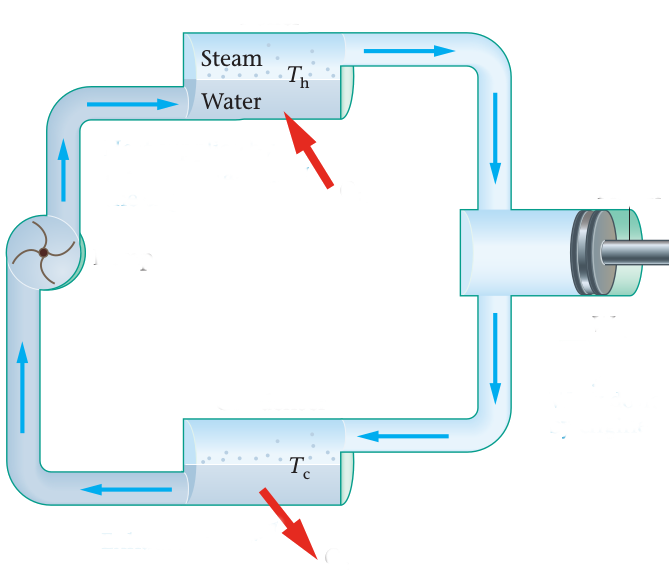
\includegraphics[scale=.3]{heat-engine}};
    		\node at (-1.7,.2) {\fontsize{10}{10}{\text{\ak ម៉ាស៊ីនបូម}}};
    		\node at (-.5,-1) {\fontsize{10}{10}{\text{\ak ករជាញើស}}};
    		\node at (-.5,3.1) {\fontsize{10}{10}{\text{\ak ឆ្នាំងដាំទឹក}}};
    		\node at (3.5,1.2) {\fontsize{10}{10}{\text{\ak ពីស្តុង}}};
    		\node at (.3,1) {$Q_{h}$};
    		\node at (.1,-2.8) {$Q_{c}$};
    		\node at (3.2,-.5) {$W$};
    		\draw (3.1,.5) -- (3.1,1.2);
    		\draw[->, line width=2pt] (2.7,-.8) -- (3.7,-.8);
    		\end{tikzpicture}
    		\caption{ម៉ាសុីនចំហាយទឹក}
    	\end{figure}
    \end{minipage}
    នៅពេលដែលពីស្តុងផ្លាស់ទីវាអាចធ្វើឲ្យកង់ស្ពឺនៃយានអាចវិលបាន(គឺបំពេញកម្មន្តទៅមជ្ឈដ្ឋានក្រៅបាន)។ បន្ទាប់ពីចាកចេញពីម៉ាសុីន ចំហាយមួយចំនួន ក៏បន្តទៅតំបន់ដែលចំហាយឲ្យករទៅជាទឹក(ប្រភពធុងត្រជាក់)។\\
    គ្រប់ម៉ាសុីនកម្តៅទាំងអស់ស្រូបកម្តៅពីប្រភពដែលមានសីតុណ្ហភាពខ្ពស់ ដើម្បីបម្លែងជាកម្មន្តមេកានិច ហើយបញ្ចេញ ឬបំភាយកម្តៅខ្លះត្រង់ប្រភពត្រជាក់ ដែលដំណើការនេះត្រូវបានធ្វើដដែលៗ ជាវដ្តនៃដំណើការ{\en(Cycle)} ដែលបង្កើតបានជាបម្លែងបិទ។ តាមច្បាប់ទីមួយទែម៉ូឌីណាមិចៈ
    \begin{flalign*}
    \Delta U = U_{2}-U_{1}=0\quad &\quad \text{ដូចនេះ}\quad W=Q\\
    \text{ដែល}\quad Q\quad \text{ជាបរិមាណកម្តៅសរុបនៃដំណើរការរបស់ម៉ាសុីន}\quad &\quad W\quad\text{ជាកម្មន្តសរុបដែលធ្វើដោយម៉ាសុីន}
    \end{flalign*}
    \begin{itemize}
    	\item \emph{\ak ដ្យាក្រាម លំហូរនៃថាមពល}\\
    	អ្វីដែលម៉ាសុីនប្រើកម្តៅទាំងអស់មានចំណុចដូចគ្នាមានដូចជាៈ
    	\begin{enumerate}[m]
    		\item ប្រភពដែលមានសីតុណ្ហភាពខ្ពស់ផ្តល់កម្តៅមួយផ្នែកសម្រាប់ធ្វើកម្មន្ត(កម្មន្តមេកានិច)។
    		\item ប្រភពដែលមានសីតុណ្ហភាពទាបគឺមានតួនាទីសម្រាប់យកចំហាយទឹកដែលសល់ក្រោយពីកម្តៅធ្វើជាកម្មន្ត\\(កម្មន្តមេកានិច) ទៅជាទឹកឡើងវិញ។
    		\item ដំណើរការរបស់ម៉ាសុីនគឺធ្វើឡើងក្នុងបម្លែងបិទ។
    	\end{enumerate}
    	\begin{minipage}[l]{.4\textwidth}
    		\begin{flalign*}
    		\text{គេមាន}\quad:&\quad W=Q\\ 
    		\text{ដែល}\quad:&\quad Q=Q_{h}-Q_{c}\\
    		\text{នោះ}\quad:&\quad W=Q_{h}-Q_{c} \\
    		\text{ដូចនេះ}\quad:&\quad W=Q_{h}-Q_{c}\quad
    		\end{flalign*}
    	\end{minipage}
    	\begin{minipage}[r]{.7\textwidth}
    		\begin{figure}[H]
    			\centering
    			\begin{tikzpicture}[>={Triangle[angle=60:1 2]}, scale=1.5]
    			\path [shading=heat]
    			(-2,2) rectangle (2,3/2) (-2,-2) rectangle (2,-3/2);
    			\draw (-2,3/2) -- (2,3/2) (-2,-3/2) -- (2,-3/2);
    			\scoped{
    				\clip (-3/2,-7/4) rectangle (3/2,7/4);
    				\draw [shading=heat] 
    				(3/4,2) -- (-3/4,2) -- (-3/4,7/4) arc (90:0:1/4) -- (-1/2,-3/2)
    				arc (360:270:1/4) -- (-3/4,-2) -- (1/4,-2) -- (1/4,-7/4) 
    				arc (270:180:1/4) -- (0,-3/2)    -- (0,1/4)   
    				arc (180:270:1/2) -- (2,-1/4)  -- (2,1/4) -- (3/4,1/4)
    				arc (270:180:1/4) -- (1/2,3/2)  arc (180:90:1/4) -- (3/4,2);
    			}
    			\path (0,2.6) node {\text{\ak ធុងក្តៅ} $T_h$} (0,-2.5) node {\text{\ak ធុងត្រជាក់} $T_c$} (0,2) node {$Q_{h}$} (-.2,-1.8) node {$Q_{c}$} (3.5,0) node {$W=Q_{h}-Q_{c}$} (2.7,1) node {\text{\ak ម៉ាសុីន}};
    			\draw [red!75,  line width=1cm/4, ->] (0,3/2) -- (0,1/2);
    			\draw [red!75,  line width=1cm/8, ->] (-1/4,-1/2) -- (-1/4,-3/2);
    			\draw [blue!75, line width=1cm/8, ->] (1,0) -- (2,0);
    			\draw (0,.2) circle (.8cm);
    			\draw[->, line width=2pt] (2,1) -- (.7,.8);
    			\end{tikzpicture}
    			\caption{ដ្យាក្រាមតាងការបម្លែងថាមពលកម្តៅ}
    		\end{figure}
    	\end{minipage}
    	\item \emph{\ak ប្រសិទ្ធភាពនៃម៉ាសុីនកម្តៅ(\en Efficiency)}
    	\begin{flalign*}
    	\text{គេមាន}\quad :&\quad W=Q_{h}-Q_{c}\\
    	\text{គេបាន}\quad :&\quad e=\frac{W}{Q_{h}}=\frac{Q_{h}-Q_{c}}{Q_{h}}\\
    	\text{ដូចនេះ}\quad :&\quad e=1-\frac{Q_{c}}{Q_{h}}
    	\end{flalign*}
    \end{itemize}
    \begin{example}
    	\begin{enumerate}[m]
    		\item ម៉ាសុីនកម្តៅមួយស្រូបកម្តៅ $200J$ ពីធុងក្តៅដើម្បីធ្វើកម្មន្ត និងបំភាយកម្តៅអស់ $160J$ ទៅធុងត្រជាក់។ គណនាទិន្នផលកម្តៅនៃម៉ាសុីន។
    		\item ម៉ាសុីនកម្តៅមួយធ្វើកម្មន្ត $9200J$ ក្នុងមួយវដ្ត ខណៈដែលវាស្រូបកម្តៅ $25.0kcal$ ពីធុងដែលមានសីតុណ្ហភាពខ្ពស់។ គណនាទិន្នផលនៃម៉ាសុីនកម្តៅនេះ។
    		\item ម៉ាសុីនមួយបញ្ចេញកម្តៅ $8200J$ ខណៈពេលដែលម៉ាសុីនធ្វើកម្មន្តបាន $2600J$។\\ គណនាទិន្នផលនៃម៉ាសុីននេះ។
    		\item ម៉ាសុីនកម្តៅមួយទទួលថាមពល $360J$ ពីធុងក្តៅ និងផ្តល់កម្មន្ត $25J$ ក្នុងវដ្តនីមួយៗ។
    		\begin{enumerate}
    			\item គណនាទិន្នផលនៃម៉ាសុីន។
    			\item គណនាកម្តៅស្រូបដោយធុងត្រជាក់ក្នុងវដ្តនីមួយៗ។
    		\end{enumerate}
    	\end{enumerate}
    \end{example}
    \subsection{សុិចកាណូ}
    \begin{biography}
    	\begin{minipage}[l]{.6\textwidth}
    		នៅឆ្នាំ ១៨២៤  លោកសាឌី កាណូបានបោះពុម្ភសៀវភៅមួយក្បាល មានចំណងជើងថា {\en("Reflections on the Motive Power of Fire")} ដែលក្នុងនោះ គាត់បានពិនិត្យពិចារណានូវបញ្ហាថាៈ\\
    		\textit{តើមានលក្ខណៈអ្វីដែលម៉ាសុីនប្រើកម្តៅអាចមានប្រសិទ្ធភាព ឬទទួលផលបានអតិបរមា?}\\
    		ដើម្បីឆ្លើយតបនឹងសំនួរនេះ យើងពិនិត្យមើលម៉ាសុីនប្រើកម្តៅ ប្រតិបត្តិការរវាងប្រភពពីរ គឺទីមួយ ប្រភពក្តៅដែលមានសីតុណ្ហភាពថេរ $T_{h}$ និងទីពី ប្រភពត្រជាក់ដែលមានសីតុណ្ហភាពថេរ $T_{c}$។
    	\end{minipage}
    	\begin{minipage}[r]{.5\textwidth}
    		\begin{figure}[H]
    			\centering
    			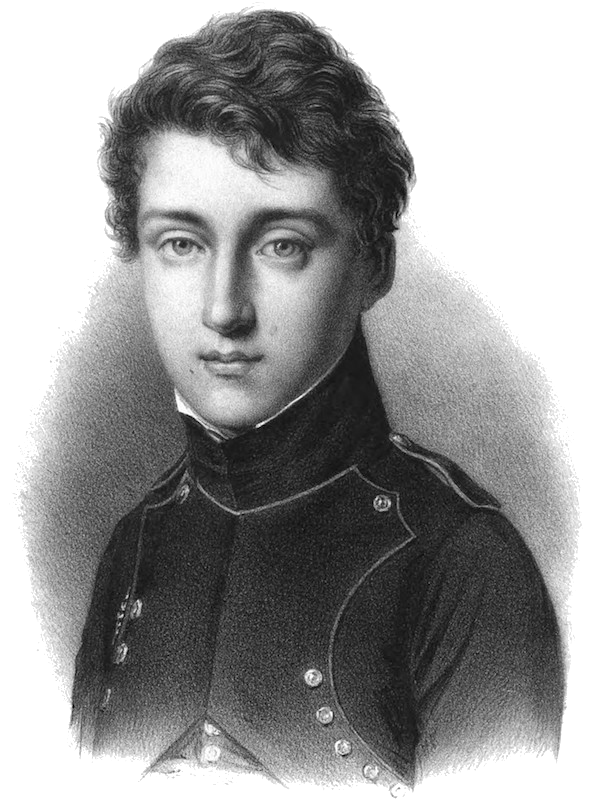
\includegraphics[scale=.15]{Nicolas-Leonard-Sadi-Carnot}\\
    			\text{\ak លោក សាឌីកាណូ}\\
    			\text{ជនជាតិបារាំង(១៧៩៦-១៨៣២)}
    		\end{figure}
    	\end{minipage}
    \end{biography}
    សុិចកាណូ ដំណើរការជាខួបរេវែសុីប{\en(Reversible)} មានបួនដំណាក់កាលដែលក្នុងនោះមាន២ជាលំនាំអុីសូទែម និង ២ទៀតជាលំនាំអាដ្យាបាទិច។\\
    ដំណើការរបស់សុិចកាណូត្រូវបានតាងលើដ្យាក្រាម $\left(PV\right)$ ដូចរូបខាងក្រោមៈ\\
    \begin{minipage}[l]{.5\textwidth}
    	\begin{itemize}
    		\item $A\rightarrow B$ ពង្រីកតាមលំនាំអុីសូទែម
    		\item $B\rightarrow C$ ពង្រីកតាមលំនាំអាដ្យាបាទិច
    		\item $C\rightarrow D$ បណ្ណែនតាមលំនាំអុីសូទែម
    		\item $D\rightarrow A$ បណ្ណែនតាមលំនាំអាដ្យាបាទិច
    	\end{itemize}
    \end{minipage}
    \begin{minipage}[r]{.6\textwidth}
    	\begin{figure}[H]
    		\centering
    		\begin{tikzpicture}[
    		> = latex,
    		dot/.style = {draw,fill,circle,inner sep=1pt},
    		arrow inside/.style = {postaction=decorate,decoration={markings,mark=at position .55 with \arrow{>}}}
    		]
    		\begin{scope}
    		\draw[<->] (0,4.5) node[left] {$P$} |- (4.5,0) node[right] {$V$};
    		\node[dot,label={above:$A$}] (@a) at (0.5,4) {};
    		\node[dot,label={right:$B$}] (@b) at (2.5,3) {};
    		\node[dot,label={right:$C$}] (@c) at (4,1) {};
    		\node[dot,label={left:$D$}] (@d) at (1.5,2) {};
    		\draw[arrow inside] (@a) to[looseness=.7,bend right=20] (@b);
    		\draw[arrow inside] (@b) to[looseness=.7,bend right=20] (@c);
    		\draw[arrow inside] (@c) to[looseness=.7,bend left=20] (@d);
    		\draw[arrow inside] (@d) to[looseness=.7,bend left=20] (@a);
    		\draw[->, line width=3pt] (2,3.5) -- (2,2.5);
    		\draw[->, line width=3pt] (2,2) -- (2,1);
    		\node[label={above:$Q_{h}$}] at (2,3.5) {};
    		\node[label={below:$Q_{c}$}] at (2,1) {};
    		\draw[dashed] (@a)--(.5,0);
    		\draw[dashed] (@b)--(2.5,0);
    		\draw[dashed] (@c)--(4,0);
    		\draw[dashed] (@d)--(1.5,0);
    		\coordinate[label=below:$V_{A}$] (VA) at (.5,0);
    		\coordinate[label=below:$V_{B}$] (VB) at (2.5,0);
    		\coordinate[label=below:$V_{C}$] (VC) at (4,0);
    		\coordinate[label=below:$V_{D}$] (VD) at (1.5,0);
    		\end{scope}
    		\end{tikzpicture}
    		\caption{ដ្យាក្រាមសុិចកាណូ}
    	\end{figure}
    \end{minipage}
    \begin{enumerate}
    	\item \emph{\ak តាមគន្លងនីមួយៗយើងអាចបកស្រាយដូចខាងក្រោម៖}
    	\begin{itemize}
    		\item [$-$] គន្លង $AB:$ ឧស្ម័នត្រូវបានរីកតាមលំនាំអុីសូទែម។ គេបាន $\Delta T=0$ នោះ $\Delta U=0$ ដែរ។\\
    		តាមច្បាប់ទី១ ទែម៉ូឌីណាមិច $Q=W+\Delta U\Rightarrow W=Q$ មានន័យថា បរិមាណកម្តៅ $Q_{h}$ ដែលបានស្រូបដោយឧស្ម័ន ពីធុងក្តៅដែលមានសីតុណ្ហភាព $T_{h}$ ស្មើនឹងកម្មន្ត $W_{AB}$ ដែលធ្វើដោយឧស្ម័នក្នុងដំណើរការនេះ។
    		\item [$-$] គន្លង $BC:$ ឧស្ម័នត្រូវបានរីកតាមលំនាំអាដ្យាបាទិច។ គេបាន $Q_{h}=Q_{c}$ នោះ $Q=0$។\\
    		តាមច្បាប់ទី១ ទែម៉ូឌីណាមិច $Q=W+\Delta U\Rightarrow W=\Delta U$ មានន័យថា ថាមពលចាំបាច់សម្រាប់ធ្វើកម្មន្ត $W_{BC}$ ដែលធ្វើឡើងដោយឧស្ម័នក្នុងដំណើរការ $BC$ បានមកពីតំហយថាមពលក្នុងនៃឧស្ម័ននោះ នៅពេលដែលឧស្ម័នថយចុះពីសីតុណ្ហភាព $T_{h}$ ទៅ $T_{c}$។
    		\item [$-$] គន្លង $CD:$ ឧស្ម័នបណ្ណែនតាមលំនាំអុីសូទែម។ គេបាន $\Delta T=0$ ហើយ $\Delta U=0$។ តាមច្បាប់ទី១ទែម៉ូឌីណាមិច $Q=W+\Delta U\Rightarrow Q=W$ មានន័យថាកម្មន្ត $W_{CD}$ ដែលធ្វើលើឧស្ម័នក្នុងគន្លង $AB$ នេះស្មើនឹងកម្តៅដែលដកចេញពីឧស្ម័ន $\left(Q_{c}\right)$ នៅសីតុណ្ហភាព $T_{c}$។
    		\item [$-$] គន្លង $DA:$ ឧស្ម័នបណ្ណែនតាមលំនាំអាដ្យាបាទិច។ គេបាន $Q_{h}=Q_{c}$ នោះ $Q=0$។\\
    		តាមច្បាប់ទី១ ទែម៉ូឌីណាមិច $Q=W+\Delta U\Rightarrow W=\Delta U$ មានន័យថា ថាមពលចាំបាច់សម្រាប់ធ្វើកម្មន្ត $W_{DA}$ ដែលធ្វើឡើងដោយឧស្ម័នក្នុងដំណើរការ $DA$ ស្មើនឹងការកើនឡើងនៃថាមពលក្នុងរបស់ឧស្ម័ន នៅពេលឧស្ម័នមានសីតុណ្ហភាពកើនឡើងពី $T_{c}$ ទៅ $T_{h}$។
    	\end{itemize}
    	\item \emph{\kml ទ្រឹស្តីបទកាណូ} បានពោលដូចតទៅៈ
    	\begin{itemize}
    		\item ម៉ាសុីន ឬម៉ូទ័រប្រើកម្តៅដែលមានប្រភពកម្តៅពីរ មានទិន្នផលកម្តៅអតិបរមាកាលណាការបញ្ចូនកម្តៅមានលំនាំរេវែសុីប{\en(Reversible Process)}។
    		\item ទិន្នផលកម្តៅមិនអាស្រ័យនឹងប្រភេទប្រភពកម្តៅ ឬលំនាំនៃសិុចរេវែសុីប{\en(Process of Reversible Cycle)} ទេ។
    		\item ទិន្នផលកម្តៅអតិបរមាអាស្រ័យតែនឹងសីតុណ្ហភាពដាច់ខាតនៃប្រភពកម្តៅ $T_{h}$ និងប្រភពត្រជាក់ $T_{c}$។
    	\end{itemize}
    	\begin{flalign*}
    	\text{យើងបានទិន្នផលកម្តៅអតិបរមា}\quad :& \quad e_{C}=\frac{\Delta T}{T_{h}}=\frac{T_{h}-T_{c}}{T_{h}}=1-\frac{T_{c}}{T_{h}}\quad\text{\en Carnot(ideal) Efficiency}
    	\end{flalign*}
    \end{enumerate}
    \subsection{ម៉ាសុីនអុីដេអាល់}
    ចំពោះម៉ាសុីនអុីដេអាល់ យើងបានកម្តៅសមាមាត្រនឹងសីតុណ្ហភាពៈ $\frac{T_{h}}{T_{c}}=\frac{Q_{h}}{Q_{c}}$
    \begin{flalign*}
    \text{គេអាចសរសេរ}\quad :&\quad e_{C}=1-\frac{Q_{c}}{Q_{h}}=\frac{Q_{h}-Q_{c}}{Q_{h}}=\frac{W}{Q_{h}}\\
    \text{ដូចនេះ}\quad :&\quad e_{C}=\frac{W}{Q_{h}}\left(\text{ជាទិន្នផលកម្តៅអតិបរមា}\right)
    \end{flalign*}
    \section{ម៉ាសុីនពិត(ម៉ាសុីនសាំង,ម៉ាសុីនម៉ាស៊ូត)}
    ម៉ូទ័រទាំងឡាយណាដែលធ្វើឲ្យកម្តៅក្លាយជាកម្មន្ត ហៅថា ម៉ូទ័រកម្តៅ ឬម៉ាសុីនកម្តៅ។ គេបានបែងចែកម៉ូទ័រចំហេះជាពីរគឺម៉ូទ័រចំហេះក្នុង និងម៉ូទ័រចំហេះក្រៅ។
    \begin{itemize}
    	\item \emph{\kml ម៉ូទ័រចំហេះក្រៅៈ} ជាប្រភេទម៉ូទ័រដែលបន្ទប់ចំហេះស្ថិតនៅក្រៅកន្លែង ដែលកម្តៅត្រូវបានធ្វើទៅជា កម្មន្ត។\\
    	ឧទាហរណ៍ៈ ម៉ាសុីនប្រើចំហាយទឹក ទួប៊ីនប្រើចំហាយទឹក។ ល។(ខ្ញុំបានបង្ហាញនៅចំណុចខាងលើរួចហើយនៃគំរូម៉ាសុីនចំហាយទឹក)
    	\item \emph{\kml ម៉ូទ័រចំហេះក្នុងៈ} ជាប្រភេទម៉ូទ័រដែលបន្ទប់ចំហេះស្ថិតនៅក្នុងកន្លែង ដែលកម្តៅត្រូវបានធ្វើទៅជា កម្មន្ត។\\
    	ឧទាហរណ៍ៈ ម៉ាសុីនសាំង ម៉ាសុីនម៉ាស៊ូត។\\
    	ម៉ូទ័រចំហេះក្នុងចែកចេញជាពីរប្រភេទទៅតាមបច្ចេកទេសនៃការឆេះរបស់ល្បាយ ប្រេងឥន្ទនៈ ខ្យល់ គឺ៖
    	\begin{itemize}
    		\item ម៉ូទ័រដែលបញ្ឆេះដោយបញ្ជា(ម៉ូទ័រសាំង)
    		\item ម៉ូទ័រដែលបញ្ឆេះដោយបណ្ណែន(ម៉ូទ័រម៉ាស៊ូត)
    	\end{itemize}
    	\subsection{ម៉ាសុីនសាំងបន្ទុះបួនវគ្គ}
    		\item \emph{\kml ម៉ូទ័រសាំងបន្ទុះបួនវគ្គ} ដំណើរការមានដូចតទៅៈ
    		\begin{itemize}
    			\item វគ្គទី១(ស្រូប ឬសម្រូប): ពិស្តុងធ្លាក់ចុះក្រោម ស៊ូបាប់ស្រូបបើកលាយល្យាយចំហាយសាំង-ខ្យល់។
    			\item វគ្គទី២(បណ្ណែន): ស៊ូបាប់ស្រូបបិទ ពិស្តុងផ្លាស់ទីឡើងលើបណ្ណែនល្បាយចំហាយសាំង-ខ្យល់។
    			\item វគ្គទី៣(បន្ទុះ និងបន្ធូ): ប៊ូសុីបញ្ចេញផ្កាភ្លើង ធ្វើឲ្យឆេះល្បាយសាំង-ខ្យល់។\\ ឧស្ម័នរីកមាឌធាក់ពិស្តុងចុះក្រោមវិញ(វគ្គនេះជាវគ្គដែលបង្កើតកម្មន្ត)
    			\item វគ្គទី៤(បញ្ចេញ): ពិស្តុងផ្លាស់ទីឡើងលើ ស៊ូប៉ាប់បញ្ចេញបើកបញ្ចេញចំហេះឧស្ម័នទៅក្រៅ។
    		\end{itemize}
    		\begin{figure}[H]
    			\centering
    			\begin{subfigure}{.2\textwidth}
    				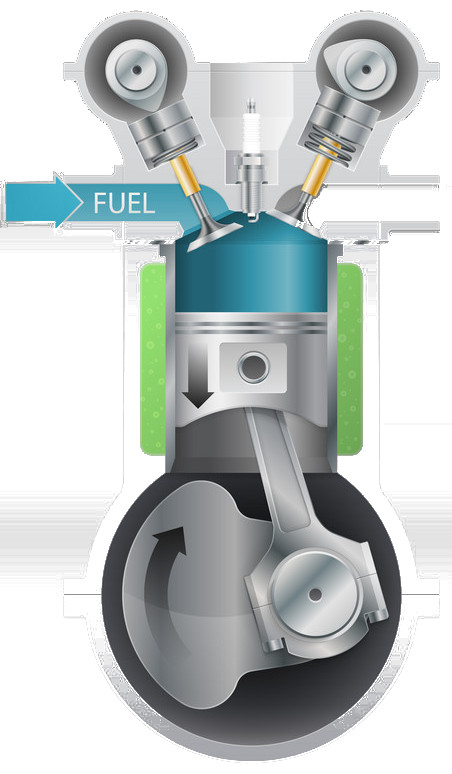
\includegraphics[scale=.2]{first-stroke}
    				\subcaption{\ak វគ្គសម្រូប}
    			\end{subfigure}
    			\begin{subfigure}{.2\textwidth}
    				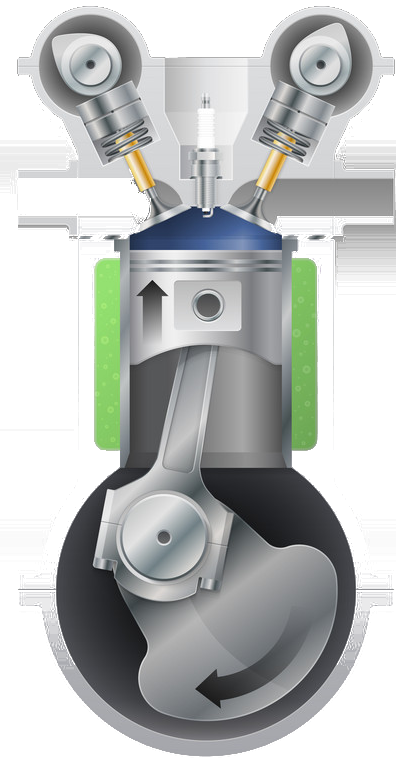
\includegraphics[scale=.2]{second-stroke}
    				\subcaption{\ak វគ្គបណ្ណែន}
    			\end{subfigure}
    			\begin{subfigure}{.2\textwidth}
    				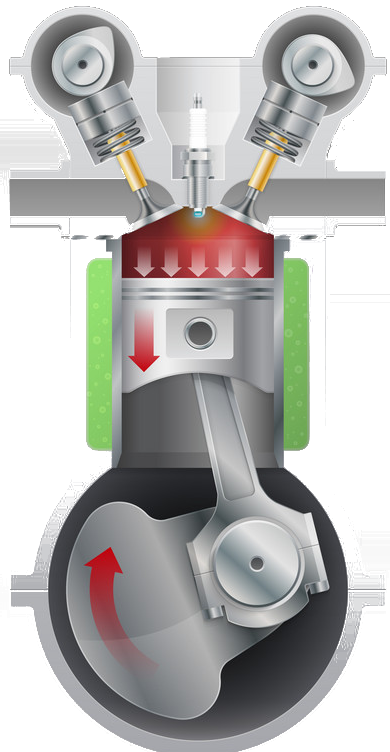
\includegraphics[scale=.2]{thirth-stroke}
    				\subcaption{\ak វគ្គបន្ទុះ និងបន្ធូ}
    			\end{subfigure}
    			\begin{subfigure}{.2\textwidth}
    				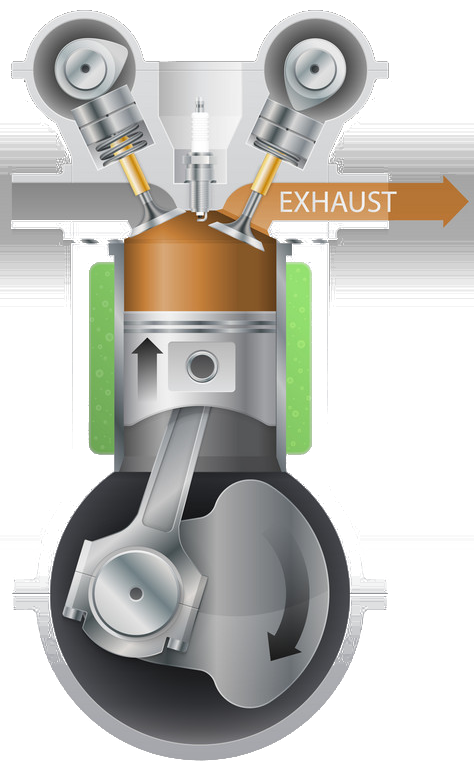
\includegraphics[scale=.2]{fourth-stroke}
    				\subcaption{\ak វគ្គបញ្ចេញ}
    			\end{subfigure}
    			\caption{ដំណើរការម៉ូទ័របន្ទុះបួនវគ្គ}
    		\end{figure}
    		\subsection{ម៉ាសុីនម៉ាស៊ូតបន្ទុះបួនវគ្គ}
    		\item \emph{\kml ម៉ូទ័រម៉ាស៊ូតបន្ទុះបួនវគ្គ} ដំណើរការមានដូចតទៅៈ 
    		\begin{itemize}
    			\item វគ្គទី១(សម្រូប): ស៊ូប៉ាប់ស្រូបបើក ពិស្តុងផ្លាស់ទីទទួលខ្យល់ធ្វើឲ្យមានកំណើនមាឌតាមលំនាំអុីសូបារ។
    			\item វគ្គទី២(បណ្ណែន): ស៊ូប៉ាប់ទាំងពីរបិទជិត ពិស្តុងផ្លាស់ទីបណ្ណែនខ្យល់ធ្វើឲ្យសម្ពាធខ្យល់កើនឡើងតាមលំនាំអុីសូទែម។
    			\item វគ្គទី៣(បន្ទុះ និងបន្ធូ): ពិស្តុងផ្លាស់ទីដល់ចំណុចដើមតាមលំនាំអុីសូបារ សីតុណ្ហភាពកើនឡើងខ្លាំង។ ប្រេងម៉ាស៊ូតក៏ត្រូវបានបាញចូល និងឆេះដោយខ្យល់ក្តៅ។ ឧស្ម័នរីកមាឌតាមលំនាំអុីសូទែម រុញពិស្តុងចេញវិញ។
    			\item វគ្គទី៤(បញ្ចេញ): ពិស្តុងផ្លាស់ទីបង្រួមមាឌឧស្ម័ន ស៊ូប៉ាប់បញ្ចេញបើក ឯប៉ាប់ស្រូបបិទធ្វើឧ្យម៉ាស៊ូតដែលឆេះស្ទុះចេញក្រៅរហូតឆេះអស់។
    		\end{itemize}
    		\subsection{ម៉ាសុីនសាំងលាយបន្ទុះពីរវគ្គ}
    		\item \emph{\kml ម៉ូទ័រសាំងលាយបន្ទុះពីរវគ្គ} ដំណើរការមានដូចតទៅៈ
    		\begin{itemize}
    			\item វគ្គទី១(បណ្ណែន និងបន្ទុះ): ពិស្តុងផ្លាស់ទីឡើងលើបិទរន្ធបញ្ចេញ ល្យាយចំហាយសាំង-ខ្យល់មួយភាគត្រូវបានបណ្ណែន។ មុនពេលពិស្តុងឡើងដល់ ចំណុចខ្ពស់បំផុត ប៊ូសុីបាញ់ភ្លើងធ្វើឧស្ម័នរីកមាឌផ្ទុះឡើង។
    			\item វគ្គទី២(ស្រូប និងបញ្ចេញ): ពិស្តុងធ្លាក់យ៉ាងរហ័សបន្ទាប់ពីផ្ទុះ។ តួពីស្តុងក៏បិទរន្ធស្រូបវិញ និងបើករន្ធបញ្ចេញពេលធ្លាកដល់ក្រោមបំផុតដែលធ្វើឲ្យឧស្ម័នអាចចេញក្រៅបាន។
    		\end{itemize}
    		\subsection{ទិន្នផលនៃម៉ាសុីនកម្តៅ}
    		\begin{itemize}
    			\item [$\bullet$] \emph{\kml ដ្យាក្រាមតុល្យភាពថាមពល}
    			\begin{figure}[H]
    				\centering
    				\begin{tikzpicture}[scale=0.9]
    				\begin{scope}
    				\filldraw[orange, fill=yellow!60!white] (0,0) circle (1.5cm);
    				\filldraw[blue, fill=blue!20!white] (6,0) circle (1.5cm);
    				\draw[->, >=latex, red!80!black, line width=10pt] (-5,0) to (-1.5,0);
    				\draw[->, >=latex, green!60!black, line width=10pt] (1.5,0) to (4.5,0);
    				\draw[->, >=latex, green!60!black, line width=10pt] (7.5,0) to (10.5,0);
    				\draw[->, >=latex, blue!60!black, line width=10pt] (0,-1.5) to (0,-4);
    				\draw[->, >=latex, blue!60!black, line width=10pt] (6,-1.5) to (6,-4);
    				\node at (0,0) {\textcolor{blue}{\ak បន្ទប់ចំហេះ}};
    				\node at (6,0) {\textcolor{blue}{\ak ភ្លៅម៉ូទ័រ}};
    				\node at (-3,1) {\text{\ak ស្រូបកម្តៅ $Q_{h}$}};
    				\node at (3,1) {\text{\ak ផ្តល់កម្មន្ត $W_{M}$}};
    				\node at (9,1) {\text{\ak ផ្តល់កម្មន្ត $W_{U}$}};
    				\node at (-1,-4.3) {\text{\ak កម្តៅភាយចេញ $Q_{c}$}};
    				\node at (5,-4.3) {\text{\ak កម្តៅភាយចេញ $Q'_{c}$}};
    				\end{scope}
    				\end{tikzpicture}
    			\end{figure}
    			ម៉ាសុីនប្រើកម្តៅចែកចេញជាពីរផ្នែកគឺ
    			\item [$\bullet$] \emph{\kml ផ្នែកកម្តៅ(ផ្នែកបម្លែងកម្តៅៈ)} ម៉ាសុីនទទួលកម្តៅ $Q_{h}$ រួចបម្លែងទៅជាកម្មន្តមេកានិច $W_{M}$ និងបញ្ចេញកម្តៅ $Q_{c}$ ទៅក្នុងបរិយាកាស។
    			\begin{enumerate}[k]
    				\item \emph{\kml តុល្យភាពថាមពល៖} $Q_{h}=W_{M}+Q_{c}$ នោះ $W_{M}=Q_{h}-Q_{c}$
    				\begin{flalign*}
    				\text{ដែល៖}\quad &\quad Q_{h}\quad \text{កម្តៅស្រូបដោយម៉ាសុីន(ថាមពលសរុប)$\left(J\right)$}\\
    				\quad &\quad W_{M}\quad\text{កម្មន្តមេកានិច$\left(J\right)$}\\
    				\quad &\quad Q_{c}\quad \text{កម្តៅភាយចេញពីម៉ាសុីន(ថាមពលខាតបង់)$\left(J\right)$}
    				\end{flalign*}
    				\item \emph{\kml ទិន្នផលកម្តៅនៃម៉ាសុីន៖} $e_{C}=\frac{W_{M}}{Q_{h}}=1-\frac{Q_{c}}{Q_{h}}$(ក្នុងបន្ទប់ចំហេះ)
    			\end{enumerate}
    			\item [$\bullet$] \emph{\kml ផ្នែកមេកានិច(ផ្នែកបញ្ចូនៈ)} កម្មន្តមេកានិច $W_{M}$ ត្រូវបានបញ្ចូនទៅជាកម្មន្តបានការ $W_{U}$ និងកម្តៅចេញពីម៉ាសុីនដោយកកិត $Q'_{c}$។
    			\begin{enumerate}[k]
    				\item \emph{\kml តុល្យភាពថាមពល៖} $W_{M}=W_{U}+Q'_{c}$
    				\begin{flalign*}
    				\quad &\quad W_{M}\quad\text{កម្មន្តមេកានិច$\left(J\right)$}\\
    				\quad &\quad W_{U}\quad \text{កម្មន្តបានការ$\left(J\right)$}\\
    				\quad &\quad Q'_{c}\quad \text{កម្តៅភាយចេញពីម៉ាសុីនដោយកកិត(ថាមពលខាតបង់)$\left(J\right)$}
    				\end{flalign*}
    				\item \emph{\kml ទិន្នផលមេកានិច ឬទិន្នផលនៃគ្រឿងបញ្ជូននៃម៉ាសុីនកម្តៅ៖} $e_{M}=\frac{W_{U}}{W_{M}}$(លើភ្លៅម៉ូទ័រ)
    				\item \emph{\kml ទិន្នផលបានការ ឬទិន្នផលសរុប(ទិន្នផលពិត)}\\
    				យើងបានទិន្នផលសរុប ឬទិន្នផលបានការនៃម៉ាសុីនគឺៈ
    				\begin{flalign*}
    				\quad &\quad e_{U}=\frac{W_{U}}{Q_{h}}\\
    				\text{ដោយ}\quad :&\quad e_{M}=\frac{W_{U}}{W_{M}}\quad \text{នោះ}\quad W_{U}=e_{M}\times W_{M}\\
    				\text{យើងបាន}\quad:&\quad e_{U}=\frac{e_{M}\times W_{M}}{Q_{h}}=e_{M}\times e_{C}\\
    				\text{ដូចនេះ}\quad :&\quad e_{U}=\frac{W_{U}}{Q_{h}}=e_{M}\times e_{C}
    				\end{flalign*}
    			\end{enumerate}
    			\item [$\bullet$] \emph{\kml អានុភាពមេកានិចរបស់ម៉ាសុីនៈ} $P=\frac{W}{t}$ ឬ $P_{M}=\frac{W_{M}}{t}$
    			\begin{flalign*}
    			\text{ដែល}\quad :&\quad P\quad \text{គិតជា} \left(W\right)\\
    			\text{និង}\quad :&\quad t\quad \text{គិតជា}\left(s\right)
    			\end{flalign*}
    		\end{itemize}
    		\begin{remark}
    			ម៉ាសុីនសាំងមានទិន្នផលប្រហែល $30\%$ រីឯទិន្នផលម៉ាសុីនម៉ាស៊ូតប្រហែល $39\%$។ ទិន្នផលនៃគ្រឿងបញ្ចូនមានតម្លែ $90\%$ និងទិន្នផលបានការមានតម្លៃប្រហែល​ $30\%$។ ទិន្នផលនេះមានតម្លៃទាប។ ក្នុងចំណុះសាំង $10$ លីត្រ មានតែ $3$ លីត្រទេដែលផ្តល់កម្មន្តបានការ។ 
    		\end{remark}
    \end{itemize}
    \begin{example}
    	\begin{enumerate}
    		\item រាលវិនាទី ម៉ូទ័ររថយន្តមួយទទួលកម្តៅ $172kJ$ ពីប្រតិកម្មនៃចំហេះល្យាយឧស្ម័ន និងបញ្ចេញមកបរិយាកាសក្រៅ $135kJ$។
    		\begin{enumerate}[1]
    			\item \begin{enumerate}[k]
    				\item រៀបរាប់វគ្គទាំងបួននៃសុិច
    				\item គណនាកម្មន្តមេកានិច ក្នុងរយៈពេល $10$ នាទី
    				\item គណនាទិន្នផលកម្តៅនៃម៉ូទ័រ
    			\end{enumerate}
    			\item ទិន្នផលគ្រឿនបញ្ចូន $92\%$។
    			\begin{enumerate}[k]
    				\item គណនាកម្មន្តបានការដែលភ្លៅម៉ូទ័របានទទួលរយៈពេល $10$ នាទី។
    				\item គណនាទិន្នផលបានការនៃម៉ាសុីន។
    			\end{enumerate}
    		\end{enumerate}
    		\item ម៉ូទ័រម៉ាស៊ូតមួយទទួលកម្តៅ $3.83MJ$។ វាមានទិន្នផលកម្តៅ $0.45$។
    		\begin{enumerate}
    			\item គណនាកម្មន្តមេកានិចដែលផ្តល់ដោយពីស្តុង
    			\item តើកម្តៅដែលបញ្ចេញទៅក្នុងបរិយាកាសមានតម្លៃប៉ុន្មាន?
    			\item ទិន្នផលគ្រឿងបញ្ចូនគឺ $0.85$។ គណនាកម្មន្តដែលទទួលដោយភ្លៅម៉ូទ័រ។
    		\end{enumerate}
    	\end{enumerate}
    \end{example}
    \begin{center}
    	{\Large \kml\color{blue} ចប់ដោយសង្ខេប!!!}
    \end{center}
	\newpage
	\section{សំណួរ លំហាត់អនុវត្តន៍ និងកិច្ចការផ្ទះ}
	\begin{enumerate}
		\item ចូរអនុវត្តច្បាប់ទី១ ទែម៉ូឌីណាមិចក្នុងលំនាំអាដ្យាបាទិច។
		\item ចូររៀបរាប់វគ្គទាំងបួននៃដំណើរការម៉ាសុីនម៉ាស៊ូត។
		\item ចូររៀបរាប់ដំណើរប្រព្រឹត្តទៅនៃសុិចកាកណូ។
		\item ដូចម្តេចដែលហៅថា ម៉ូទ័រចំហេះក្រៅ? ម៉ូទ័រចំហេះក្នុង?
		\item ធ្វើដូចម្តេចដើម្បីតម្លើងទិន្នផលម៉ាសុីនកម្តៅ?
		\item ម៉ាសុីនកាកណូ ៣ $\left(a,b,c\right)$ ដំណើរការចន្លោះសីតុណ្ហភាពៈ $(a) 400K$ និង $500K$ $\left(b\right) 500K$ និង $600K$ $\left(c\right) 400K$ និង $600K$។ ម៉ាសុីននីមួយៗស្រូបបរិមាណកម្តៅដូចៗគ្នាពីធុងក្តៅរាល់សុិច។ ចូររៀបតម្លៃកម្មន្តដែលធ្វើដោយម៉ាសុីនទាំងបីតាមលំដាប់ពីធំទៅតូច។
		\item តើប្រភពក្តៅ និងប្រភពត្រជាក់របស់ម៉ាសុីនសាំងបន្ទុះបួនវគ្គស្ថិតនៅត្រង់តំបន់ណា? ចូរពន្យល់?
		\item កម្មន្តដែលធ្វើលើឧស្ម័នក្នុងរយៈពេលនៃលំនាំអាដ្យបាទិចគឺ $140J$។ គណនាកំណើនថាមពលក្នុងនៃប្រព័ន្ធជាកាឡូរី។
		\item ម៉ាសុីនអុីដេអាល់មួយបានបំពេញកម្មន្ត $300J$។ យើងដឹងថាម៉ាសុីនបានបញ្ចេញកម្តៅទៅមជ្ឈដ្ឋានក្រៅ $600J$។ តើម៉ាសុីននោះមានទិន្នផលប៉ុន្មាន?
		\item ម៉ាសុីនកាកណូស្រូបកម្តៅ $1200cal$ ក្នុងរយៈពេលមួយសុិចនិងដំណើរការនៅចន្លោះសីតុណ្ហភាព $500K$ និង $300K$។
		\begin{enumerate}
			\item គណនាទិន្នផលនៃម៉ាសុីន។
			\item គណនាកម្តៅដែលម៉ាសុីនបានបញ្ចេញចោល។
			\item គណនាកម្មន្តដែលបានធ្វើក្នុងរយៈពេលមួយសិុចជាស៊ូល។
		\end{enumerate}
		\item ម៉ាសុីនកាកណូមានដំណើរការនៅចន្លោះសីតុណ្ហភាព $T_{h}=850K$ និង $T_{c}=300K$។ ក្នុងសុិចនីមួយៗម៉ាសុីនបានបំពេញកម្មន្ត $1200J$ ក្នុងរយៈពេល $0.25s$។
		\begin{enumerate}
			\item គណនាទិន្នផលនៃម៉ាសុិន។
			\item គណនាតម្លៃមធ្យមនៃអានុភាពរបស់ម៉ាសុីន។
			\item គណនាបរិមាណកម្តៅដែលផ្តល់ដោយធុងដែលមានសីតុណ្ហភាពខ្ពស់។
			\item គណនាបរិមាណកម្តៅដែលផ្តល់ដោយធុងដែលមានសីតុណ្ហភាពទាប។
		\end{enumerate}
		\item ម៉ូទ័រសាំងនៃរថយន្តរេណូល{\en(Renault)} បានទទួលកម្តៅ $2\times10^{5}J/s$ ដើម្បីឲ្យមានបន្ទុះក្នុងកាប៊ុយរ៉ង់។ វាបានបញ្ចេញកម្តៅ $1.3\times10^{5}J/s$ ទៅមជ្ឈដ្ឋានក្រៅ។
		\begin{enumerate}
			\item គណនាកម្មន្តដែលធ្វើដោយពិស្តុងក្នុងរយៈពេល $1$ វិនាទី។
			\item គណនាទិន្នផលកម្តៅនៃម៉ាសុីន។
			\item គេដឹងថាទិន្នផលមេកានិចគឺ $0.85$។ គណនាកម្មន្តដែលភ្លៅម៉័ទ័របានទទួលក្នុងរយៈពេល $1$ វិនាទី។
		\end{enumerate}  
		\item គណនាកម្មន្តអតិបរមាដែលម៉ាសុីនកាកណូមួយអាចបង្កើតឡើងពេលវាទទួលកម្តៅ $1kcal$ បើវាស្រូបកម្តៅនៅសីតុណ្ហភាព $427^\circ C$ និងបញ្ខេញនៅ $177^\circ C$។
		\item ម៉ាសុីនមួយបញ្ចេញកម្តៅ $8200J$ ខណៈពេលដែលម៉ាសុីនធ្វើកម្មន្តបាន $2600J$។ គណនាទិន្នផលនៃម៉ាសុីននេះ។
		\item ម៉ាសុីនកម្តៅមួយទទួលថាមពល $360J$ ពីធុងក្តៅ និងផ្តល់កម្មន្ត $25J$ ក្នុងវគ្គនីមួយៗ។
		\begin{enumerate}
			\item គណនាទិន្នផលនៃម៉ាសុីន។
			\item គណនាកម្តៅស្រូបដោយធុងត្រជាក់ក្នុងវដ្តនីមួយៗ
		\end{enumerate}
		\item ម៉ាសុីនមួយមានទិន្នផលកម្តៅ $30\%$។ គណនា៖
		\begin{enumerate}
			\item កម្មន្តដែលបានធ្វើ ប្រសិនបើវាស្រូបកម្តៅ $150J$ ពីធុងក្តៅ។
			\item កម្តៅភាយចេញទៅធុងត្រជាក់ក្នុងវដ្តនីមួយៗ។
		\end{enumerate}
		\item ម៉ាសុីនកាកណូធ្វើការរវាងធុងក្តៅពីរនៅសីតុណ្ហភាព $500K$ និង $300K$។ 
		\begin{enumerate}
			\item រកទិន្នផលកម្តៅនៃម៉ាសុីនកាកណូ។
			\item បើវាស្រូបកម្តៅ $200kJ$ ពីធុងក្តៅ។ គណនាកម្មន្តដែលបានធ្វើ។
		\end{enumerate}
		\item ម៉ាសុីនកម្តៅមយមានអានុភាព $580MW$។ គណនាកម្តៅដែលម៉ាសុីនបាត់បង់រាល់វិនាទី បើគេដឹងថាម់ាសុីនមានទិន្នផល $32\%$។
		\item ម៉ូទ័រម៉ាសុីនម៉ាស៊ូតនៃរថយន្តមួយដែលមានទិន្នផលកម្តៅ $0.43$ ហើយស្រូបកម្តៅ $4.0MJ$ ពីប្រភពក្តៅ។\\គណនាៈ
		\begin{enumerate}
			\item កម្មន្តមេកានិចដែលបានពីពិស្តុង។
			\item បរិមាណកម្តៅដែលបញ្ចេញទៅក្នុងបរិយាកាស។
			\item កម្មន្តបានការ បើគេដឹងថាទិន្នផលគ្រឿងបញ្ចូន $0.82$។
		\end{enumerate} 
		\item ម៉ាសុីនកាកណូដែលមានអានុភាព $500W$ ដំណើរការចន្លោះសីតុណ្ហភាព $100^\circ C$ និង $60^\circ C$។ 
		\begin{enumerate}
			\item គណនាថាមពលកម្តៅស្រូបដោយម៉ាសុីនរាល់វិនាទី។
			\item គណនាកម្តៅបញ្ចេញដោយម៉ាសុីនរាល់វិនាទី។
		\end{enumerate}
		\item ម៉ាសុីនកាកណូដំណើរការនៅចន្លោះធុងកម្តៅពីរដែលមានសីតុណ្ហភាព $235^\circ C$ និង $115^\circ C$ ដោយស្រូបកម្តៅ $6.30\times10^{4}J$ រាល់វដ្តពីធុងក្តៅ។
		\begin{enumerate}
			\item គណនាទិន្នផលនៃម៉ាសុីន។
			\item គណនាកម្មន្តដែលម៉ាសុីនបានបំពេញ។
		\end{enumerate}
		\item ម៉ាសុីនម៉ាស៊ូតនៃរថយន្តមួយមានទិន្នផលកម្តៅ $0.40$ ហើយវាស្រូបបរិមាណកម្តៅ $6.0\times10^{6}J$។ គណនាៈ
		\begin{enumerate}
			\item កម្មន្តមេកានិចដែលបានពីពិស្តុង។
			\item បរិមាណកម្តៅដែលបញ្ចេញទៅក្នុងបរិយាកាស។
			\item កម្មន្តបានការ បើទិន្នផលគ្រឿងបញ្ជូនស្មើនឹង $0.8$។
		\end{enumerate}
		\item ម៉ាសុីនអុីដេអាល់មួយដំណើរការនៅចន្លោះធុងកម្តៅពីរដែលមានសីតុណ្ហភាព $500K$ និង $400K$ វាស្រូបកម្តៅ $10.0\times10^{2}J$ ពីធុងដែលមានសីតុណ្ហភាពខ្ពស់ក្នុងរយៈពេលសិុចនីមួយៗ។
		\begin{enumerate}
			\item គណនាទិន្នផលរបស់ម៉ាសុីននោះ។
			\item តើកម្តៅដែលម៉ាសុីនបញ្ចេញទៅមជ្ឈដ្ឋានក្រៅមានតម្លៃប៉ុន្មាន?
		\end{enumerate}
		\item កម្មន្តដែលបំពេញដោយម៉ាសុីនមួយស្មើនឹង $1/4$ នៃកម្តៅស្រូបពីធុងក្តៅ។
		\begin{enumerate}
			\item គណនាទិន្នផលអតិបរមានៃម៉ាសុីន។
			\item តើម៉ាសុីនខាតបង់កម្តៅប៉ុន្មានភាគរយ។
		\end{enumerate}
		\item ម៉ូទ័រម៉ាស៊ូតមួយទទួើលកម្តៅ $3.83MJ$។ វាមានទិន្នផលកម្តៅ $0.45$។
		\begin{enumerate}
			\item គណនាកម្មន្តមេកានិចដែលផ្តល់ដោយពិស្តុង។
			\item តើកម្តៅដែលបញ្ចេញទៅក្នុងបរិយាកាសមានតម្លៃប៉ុន្មាន?
			\item ទិន្នផលគ្រឿងបញ្ចូនគឺ $0.85$។
			គណនាកម្មន្តដែលបញ្ចូនដោយភ្លៅម៉ូទ័រ។
		\end{enumerate}
		\item ម៉ាសុីនកម្តៅមួយមានអានុភាពចេញ $5.00kW$ និងមានទិន្នផល $25\%$។ ម៉ាសុីនបានបំភាយកម្តៅ $8.00\times10^{3}J$ រាល់វដ្តនីមួយៗ។
		\begin{enumerate}
			\item គណនាកម្តៅស្រូបដោយម៉ាសុីនរាល់វដ្តនីមួយៗ។
			\item គណនារយៈពេលក្នុងមួយវដ្តនៃដំណើរការ។
		\end{enumerate}
		\item ម៉ាសុីនកម្តៅមួយស្រូបកម្តៅ $360J$ ពីធុងក្តៅ និងបំពេញកម្មន្ត $25.0J$ ក្នុងវដ្តនីមួយៗ។
		\begin{enumerate}
			\item គណនាទិន្នផលនៃម៉ាសុីន។
			\item គណនាកម្តៅភាយទៅធុងត្រជាក់។
		\end{enumerate}
		\item សីតុណ្ហភាពនៅក្នុងធុងត្រជាក់នៃម៉ាសុីនកាណូគឺ $230^\circ C$។ គណនាសីតុណ្ហភាពនៅក្នុងធុងក្តៅ បើម៉ាសុីនមានទិន្នផល $34\%$។
		\item ម៉ាសុីនកាណូមួយដំណើរការចន្លោះសីតុណ្ហភាព $210^\circ C$ និង $45^\circ C$។ អានុភាពចេញរបស់វាគឺ $910W$។\\ គណនាកម្តៅភាយចេញពីម៉ាសុីនរាល់វិនាទី។
		\item ម៉ាសុីនកាណូមួយមានទិន្នផល $22\%$។ វាដំណើរការចន្លោះធុងកម្តៅពីរដែលមានបម្រែបម្រួលសីតុណ្ហភាព $75.0^\circ C$។
		\begin{enumerate}
			\item គណនាសីតុណ្ហភាពក្នុងធុងក្តៅ។
			\item គណនាសីតុណ្ហភាពក្នុងធុងត្រជាក់។
		\end{enumerate}
		\item ម៉ាសុីនកាកណូមួយមានអានុភាព $520kW$ ដោយស្រូបកម្តៅ $950kcal$ រាល់វិនាទី។ ប្រសិនបើសីតុណ្ហភាពប្រភពក្តៅ $520^\circ C$ ចូរគណនាសីតុណ្ហភាពប្រភពត្រជាក់។
		\item ម៉ាសុីនសាំងមួយដែលមានសុីឡាំងចំនួនបួនមានទិន្នផល $0.22$ និងបំពេញកម្មន្តបាន $180J$ រាល់ជុំក្នុងសុីឡាំងនីមួយៗ។ ប្រសិនបើម៉ាសុីនដំណើរការបាន $25\mathbf{rps}$។
		\begin{enumerate}
			\item គណនាកម្មន្តបំពេញក្នុងមួយវិនាទី។
			\item គណនាកម្តៅសរុបដែលផ្តលឲ្យម៉ាសុីនក្នុងមួយវិនាទី។
			\item ប្រសិនបើចំហេះសាំង $1\ell$ ផ្តល់ថាមពលបាន $32.21MJ$។\\ តើក្នុងសាំងមួយលីត្រអាចប្រើបានក្នុងរយៈពេលប៉ុន្មាន។
		\end{enumerate}
		\item ម៉ាសុីនកម្តៅទី $1$ ទទួលកម្តៅធំជាងម៉ាសុីនទី $2$ បួនដង បានបំពេញកម្មន្តពីរដង និងបញ្ចេញកម្តៅប្រាំពីរដងនៃម៉ាសុីនទី $2$ ទៅធុងត្រជាក់វិញ។ គណនាទិន្នផលនៃម៉ាសុីនទាំងពីរ។
		\item ម៉ាសុីនកាណូមួយដំណើរការចន្លោះសីតុណ្ហភាព $293K$ និង $67K$។ តើវិធីសាស្រ្តណាមួយដែលធ្វើឲ្យទិន្នផលនៃម៉ាសុីនកើនឡើងខ្ពស់ជាង "បង្កើនសីតុណ្ហភាព $10^\circ C$ នៅក្នុងធុងក្តៅ" ឬក៏ "បន្ថយសីតុណ្ហភាព $10^\circ C$ នៅក្នុងធុងត្រជាក់"? ចូរបង្ហាញហេតុផលសាមញ្ញមួយ។
		\item ម៉ាសុីនកម្តៅបញ្ចេញកម្តៅទៅកាន់ធុងដែលមានសីតុណ្ហភាព $340^\circ C$ និងមានទិន្នផលទ្រឹស្តី $36\%$។ តើធុងត្រជាក់មានសីតុណ្ហភាពប៉ុន្មានអង្សា ប្រសិនបើម៉ាសីុនកើនទិន្នផលដល់ $42\%$ និងរក្សាសីតុណ្ហភាពក្នុងប្រភពក្តៅដដែល។
		\item ម៉ាសុីនកាណូមួយដំណើរការចន្លោះប្រភពកម្តៅដែលមានសីតុណ្ហភាព $580^\circ C$ និងមានទិន្នផលអតិបរមា $22\%$។ ដើម្បីបង្កើនទិន្នផលម៉ាសុីនដល់ $42\%$ តើគេត្រូវតម្លើងសីតុណ្ហភាពប្រភពក្តៅដល់ប៉ុន្មានអង្សា បើសីតុណ្ហភាពប្រភពត្រជាក់ត្រូវរក្សា?
		\item ម៉ាសុីនកាណូមួយមានធុងត្រជាក់ដែលមានសីតុណ្ហភាព $17^\circ C$ មានទិន្នផល $40\%$។ តើគេត្រូវតម្លើងសីតុណ្ហភាព ប្រភពក្តៅប៉ុន្មានដើម្បឲ្យទិន្នផលរបស់ម៉ាសុីនកើនដល់ $50\%$។\\ ដោយដឹងថាសីតុណ្ហភាពប្រភពត្រជាក់ត្រូវបានរក្សា។
		\item ម៉ាសុីនកាណូមួយប្រើចំហាយទឹកក្តៅ $100^\circ C$ ដែលជាធុងក្តៅ។ រីឯធុងត្រជាក់គឺជាមជ្ឈដ្ឋានខាងក្រៅ ដែលមានសីតុណ្ហភាព $20^\circ C$។ អត្រាថាមពលដែលត្រូវបានបញ្ចូនទៅកាន់ធុងត្រជាក់មាន $15.4W$។
		\begin{enumerate}
			\item គណនាអានុភាពបានការនៃម៉ាសុីនកម្តៅ។
			\item គណនាចំហាយកំណជាទឹកនៅធុងក្តៅក្នុងរយៈពេល $1.00h$ ហើយកម្តៅឡាតង់ដើម្បីឲ្យចំហាយកំណជាទឺក $L=2.26\times10^{6}J/kg$។
		\end{enumerate}
		\item ម៉ាសុីនកម្តៅមួយ ត្រូវបានតភ្ជាប់ទៅធុងកម្តៅពីរដែលមួយជាអាលុយមីញ៉ូមរលាយនៅសីតុណ្ហភាព $660^\circ C$ និងធុងមួយទៀត គឺដុំបារតនៅសីតុណ្ហភាព $-38.9^\circ C$។ ម៉ាសុីនដំណើរការដោយបង្កកអាលុយមីញ៉ូម $1.0g$ និងរំលាយបារត $15.0g$។ គេដឹងថា បន្សាយកម្តៅម៉ាសអាលុយមីញ៉ូម $3.97\times10^{5}J/kg$ និងបន្សោយកម្តៅម៉ាសបារត $1.18\times10^{4}J/kg$។ គណនាទិន្នផលអតិបរមានៃម៉ាសុីន។
		\item ម៉ាសុីនកាណូប្រើចំហាយទឹកមួយចាប់ផ្តើមដំណើរការរវាងសីតុណ្ហភាពចំហាយ $220^\circ C$ និងសីតុណ្ហភាព $35^\circ C$ ដោយផ្តល់នូវអានុភាព $8hp$(សេះ)។ គណនាកម្តៅស្រូបក្នុងមួយវិនាទីដោយម៉ាសុីនចំហាយ និងកម្តៅបញ្ចេញក្នុងមួយវិនាទីគិតជាកាឡូរី។ បើម៉ាសុីនកាណូដំណើរការរវាងសីតុណ្ហភាពកម្រិតទាំងនេះមានទិន្នផល $30\%$ នៃទិន្នផលកម្តៅ។
		\item ម៉ាសុីន $X$ បានទទួលថាមពលកម្តៅពីធុងដែលមានសីតុណ្ហភាពខ្ពស់ $4$ដងធំ ជាងម៉ាសុីន $Y$។ ម៉ាសុីន $X$ បានធ្វើកម្មន្ត $2$ដង ហើយបានបញ្ចេញថាមពលកម្តៅ $7$ដងដោយធុងដែលមានសីតុណ្ហភាពទាបធំជាងម៉ាសុីន $Y$។
		\begin{enumerate}
			\item គណនាទិន្នផលម៉ាសុីនកម្តៅ $Y$។
			\item គណនាទិន្នផលម៉ាសុីនកម្តៅ $X$។
		\end{enumerate}
		\item សុីឡាំងច្រើនរបស់ម៉ាសុីនសាំងយន្តហោះមួយដំណើរការដោយល្បឿន $2500\mathbf{tr/mn}$ ដោយទទួលថាមពលកម្តៅ $7.89\times10^{3}J$ និងបញ្ចេញថាមពលកម្តៅ $4.58\times10^{3}J$ ក្នុងជុំនីមួយៗនៃម៉ាសុីនយន្តហោះវីឡឺ​​​ប្រឺ​​កាំង។
		\begin{enumerate}
			\item គណនាប្រេងសាំងគិតជាលីត្រក្នុងរយៈពេល $1$ម៉ោងនៃដំណើរការ។\\ ប្រសិនបើកម្តៅចំហេះនៃសាំង $4.03\times10^{7}J/L$។
			\item គណនាអានុភាពមេកានិចដែលម៉ាសុីនផលិតបាន។
			\item គណនាម៉ូម៉ង់ដែលម៉ាសុីនយន្តហោះប្រើលើបន្ទុក។
			\item គណនាអានុភាពមិនបានការដែលបានបញ្ចេញដោយធុងសីតុណ្ហភាពទាប។
		\end{enumerate}
		\item ម៉ាសុីនកាណូមួយផលិតអានុភាពបានការ $150kW$។ ម៉ាសុីននេះបានដំណើរការរវាងសីតុណ្ហភាពពីរគឺ $20^\circ C$ និង $500^\circ C$។
		\begin{enumerate}
			\item គណនាថាមពលជាកម្តៅដែលវាទទួលបានក្នុងរយៈពេល $1$ម៉ោង។
			\item គណនាថាមពលជាកម្តៅដែលវាបាត់បង់ក្នុងរយៈពេល $1$ម៉ោង។
		\end{enumerate}
		\item ម៉ាសុីនកាណូមួយមានអានុភាព $P$។ ម៉ាសុីននេះបានដំណើរការរវាងដំណើរការរវាងសីតុណ្ហភាពពីរគឺ $T_{h}$ និង $T_{c}$។
		\begin{enumerate}
			\item គណនាថាមពលជាកម្តៅដែលចូលក្នុងម៉ាសុីននៅចន្លោះពេល $\Delta t$។
			\item គណនាថាមពលជាកម្តៅដែលបាត់ប៉ង់ក្នុងចន្លោះពេល $\Delta t$។
		\end{enumerate}
		\item ម៉ាសុីនមួយបានបញ្ចូនថាមពលជាកម្តៅ $2\times10^{3}J$ ពីប្រភពធុងសីតុណ្ហភាពខ្ពស់ក្នុងអំឡុងខួបនីមួយៗហើយបានបញ្ចូន $1.5\times10^{3}J$ ទៅប្រភពសីតុណ្ហភាពទាប។
		\begin{enumerate}
			\item គណនាទិន្នផលរបស់ម៉ាសុីន។
			\item គណនាកម្មន្តដែលធ្វើដោយម៉ាសុីនក្នុង $1$ខួប។
			\item គេដឹងថា ម៉ាសុីននេះដំណើរការដោយល្បឿន $2000\mathbf{tr/mn}$។\\
			គណនាអានុភាពមេកានិចដែលម៉ាសុីននោះផលិតបានក្នុង $1$ជុំ។
		\end{enumerate}
		\item កម្មន្តដែលធ្វើដោយម៉ាសុីនស្មើ $1/4$ នៃថាមពលកម្តៅដែលស្រូបចេញពីធុងសីតុណ្ហភាពខ្ពស់។
		\begin{enumerate}
			\item គណនាទិន្នផលកម្តៅរបស់ម៉ាសុីន។
			\item គណនាផលធៀបថាមពលដែលស្រូបនិងថាមពលដែលបញ្ចេញទៅធុងសីតុណ្ហភាពទាប។
		\end{enumerate}
		\item កាំភ្លើងមយយត្រូវបានចាត់ទុកជាម៉ាសុីនកម្តៅ។ គេដឹងថាកាំភ្លើងធ្វើពីដែកដែលមានម៉ាសស្មើ $1.8kg$។ គ្រាប់កាំភ្លើងនេះមានម៉ាស $2.40g$ ហើយពេលបាញ់ចេញមានល្បឿន $320m/s$ និងមានទិន្នផលថាមពលស្មើ $1.10\%$។ សន្មតថាតួ(ដង)កំាភ្លើងស្រូបថាមពលទាំងអស់ដែលបញ្ចេញនិងកើនឡើងសីតុណ្ហភាពស្មើសាច់ក្នុងរយៈពេលខ្លឺមុនពេលបាត់បង់ថាមពលកម្តៅខ្លះទៅក្នុងមជ្ឈដ្ឋានបរិយាកាស។\\ គណនាកំណើនសីតុណ្ហភាពនៅក្នុងគ្រាប់កាំភ្លើង។ គេឲ្យកម្តៅម៉ាសដែក $C_{\text{ដែក}}=448J/kg^{\circ}C$។
		\item ម៉ាសុីនមួយកើតឡើងពីចំហេះធ្យូងថ្មបង្វិលតួប៊ីននៅជ្រលងស្ទឹង(អូហាយអូ) នៅសហរដ្ឋអាមេរិចដែលដំណើរការរវាងសីតុណ្ហភាពពីរ $1870^\circ C$ និង $430^\circ C$។
		\begin{enumerate}
			\item តើទិន្នផលម៉ាសុីនទ្រឹស្តីអតិបរមាស្មើប៉ុន្មាន?
			\item ទិន្នផលម៉ាសុីនពិតស្មើ $42\%$។ គណនាអនុភាពមេកានិចដែលម៉ាសុីនបានបញ្ចូន ប្រសិនវាស្រូបថាមពលកម្តៅ $1.40\times10^{5}J$ រៀងរាល់វិនាទីពីធុងសីតុណ្ហភាពខ្ពស់។
		\end{enumerate}
		\item ម៉ាសុីនកម្តៅមយយបង្កើតឡើងមានទិន្នផលស្មើម៉ាសុីនកាណូ $65\%$ នៅពេលវាដំណើរការរវាងធុងសីតុណ្ហភាពពីរ។
		\begin{enumerate}
			\item ប្រសិនបើសីតុណ្ហភាពធុងត្រជាក់ស្មើនឹង $20^\circ C$ តើសីតុណ្ហភាពដែលនៅធុងដែលមានសីតុណ្ហភាពខ្ពស់ស្មើប៉ុន្មាន?
			\item តើទិន្នផលម៉ាសុីនពិតអាចស្មើ $65\%$ ដែរឬទេ? ចូរពន្យល់?
		\end{enumerate}
		\item ក្នុងភាពទី១នៃភាពពីររបស់ម៉ាសុីនកាណូមួយថាមពលដែលស្រូប $Q_{1}$ ក្រោមសីតុណ្ហភាព $T_{1}$ ហើយធ្វើកម្មន្ត $W_{1}$ និងបញ្ចេញថាមពលកម្តៅ $Q_{2}$ ក្រោមសីតុណ្ហភាពទាប $T_{2}$។ ភាពទី២ ស្រូបថាមពលកម្តៅ $Q_{2}$ ធ្វើកម្មន្ត $W_{2}$ ហើយបញ្ចេញថាមពលកម្តៅ $Q_{3}$ ក្រោមសីតុណ្ហភាព $T_{3}$។\\
		ចូរបង្ហាញថា ទិន្នផលរបស់ម៉ាសុីនកម្តៅនេះគឺ $e=\frac{T_{1}-T_{3}}{T_{1}}=1-\frac{T_{3}}{T_{1}}$។ 
		\item ទិន្នផលនៃម៉ាសុីនពិត $20\%$ គឺប្រើដើម្បីបង្កើនល្បឿនរបស់រថភ្លើងមួយចេញពីស្ងៀមទៅល្បឿនប្រហែល $5m/s$។ យើងដឹងដា ម៉ាសុីនកាណូមួយបានប្រើប្រភពធុងត្រជាក់និងធុងក្តៅដូចគ្នាដើម្បីពន្លឿនរថភ្លើងដូចគ្នាពីនៅស្ងៀមទៅល្បឿន $6.50m/s$ ដោយប្រើបរិមាណបេ្រងឥន្ធនៈស្មើគ្នា។ ម៉ាសុីននេះប្រើខ្យល់ដែលមានសីតុណ្ហភាព $300K$ ធ្វើជាប្រភពធុងត្រជាក់។
		គណនាសីតុណ្ហភាពនៃចំហាយដែលប្រើនៅប្រភពធុងក្តៅ។
		\item ក្នុងមួយខួប ម៉ាសុីនកម្តៅមួយបានស្រូប $500J$ ពីធុងដែលមានសីតុណ្ហភាពខ្ពស់ហើយបញ្ចេញ $300J$ ទៅប្រភពធុងសីតុណ្ហភាពទាប។ គេដឹងថាទិន្នផលម៉ាសុីនស្មើនឹង $60\%$ នៃម៉ាសុីនកាណូ។ គណនាផលធៀបសីតុណ្ហភាពធុងត្រជាក់ និងសីតុណ្ហភាពធុងក្តៅនៃម៉ាសុីនកាណូ។
		\item ម៉ាសុីនកាណូមួយបានដំណើរការរវាងសីតុណ្ហភាព $T_{h}=100^\circ C$ និង $T_{c}=20^\circ C$។ តើផលធៀបទិន្នផលនៃម៉ាសុីនកាណូនេះកើនឡើងស្មើនឹងប៉ុន្មាន? បើសីតុណ្ហភាពធុងក្តៅកើនឡើងដល់ $550^\circ C$។
		\item $1500kW$ នៃម៉ាសុីនកម្តៅមួយបានដំណើរការដោយទិន្នផល $20\%$។ ថាមពលកម្តៅបានបញ្ចេញទៅធុងត្រជាក់ដោយការស្រូបចំហាយទឹកចូលក្នុងរបុំមានសិតុណ្ហភាព $20^\circ C$។ ប្រសិនបើទឹក $60$លីត បានហូរឆ្លងកាត់របុំក្នុង១វិនាទី។\\ តើកំណើនសីតុណ្ហភាពទឹកស្មើនឹងប៉ុន្មាន? គេឲ្យកម្តៅម៉ាសទឹក $C=4186J/kg^\circ C$។ ម៉ាសមាឌទឹក $\rho=10^{3}kg/m^{3}$។
		\item ម៉ាសុីនកាណូមួយបានដំណើរការរវាងសីតុណ្ហភាពពីរគឺ $100^\circ C$ និង $20^\circ C$។
		គណនាម់ាសទឹកកកដែលអាចឲ្យម៉ាសុីនរំលាយបន្ទាប់ពីវាធ្វើកម្មន្ត $5\times10^{4}J$។ គេឲ្យកម្តៅឡាតង់របស់ទឹកកក $L_{f}=3.33\times10^{5}J/kg$
		\item ម៉ាសុីនកាណូមួយមានសីតុណ្ហភាពធុងត្រជាក់ $17^\circ C$ និងមានទិន្នផល $40\%$។ តើសីតុណ្ហភាពធុងក្តៅកើនប៉ុន្មានដើម្បីឲ្យបានទិន្នផលរបស់ម៉ាសុីនកើនបាន $50\%$?
		\item ម៉ាសុីនកាណូមួយបានស្រូបថាមពលកម្តៅ $52kJ$ ហើយបានបញ្ចេញថាមពលកម្តៅ $36kJ$ ក្នុងខួបនីមួយៗ។
		\begin{enumerate}
			\item គណនាទិន្នផលរបស់ម៉ាសុីនកាណូ។
			\item គណនាកម្មន្តដែលបំពេញបានក្នុងខួបនីមួយៗ។
		\end{enumerate}
	\end{enumerate}